\section{Contexto en RASimAs}
\label{art:rasimas}

% El \ac{WP} 3 del proyecto \ac{RASimAs} tiene como objetivo crear \nuevo{un} modelo virtual con anatomía especifica de pacientes. Con el objetivo de conseguir el máximo realismo posible, se propone como objetivo crear modelos virtual que pueda usarse en el simulador que contenga anatomía real de pacientes. Para ello se propone crear la herramienta \ac{TPTVPH}.
% Este juego de herramientas está diseñado para permitir crear un \ac{VPH} y que pueda ser posicionado y movido durante su uso en el simulador.

% Para lo cual, debido a su complejidad el \ac{WP} se divide en varias tareas.
% \begin{itemize}
%     \item Tarea 3.1 Adquisición de datos:
%         A partir de imágenes de \ac{IRM}, \ac{TC}, etc... se conseguirá un modelo virtual que servirá como entrada para las tareas siguientes.
%     \item Tarea 3.2 Modelado anatómico:
%         Finalización de los modelos superficiales de los tejidos que se han recuperado de la tarea anterior.
%     \item Tarea 3.3 Modelado mecánico:
%         El objetivo es conseguir o modelar el comportamiento mecánico de los tejidos como los músculos 
%     \item Tarea 3.4 Modelado fisiológico:
%         Esta tarea está focalizada en crear el comportamiento de los nervios y el consecuente movimiento de los músculos. 
%     \item Tarea 3.5 Integración:
%         Con el resultado de todas las tareas anteriores, es posible automatizar y crear una herramienta para que partiendo de las imágenes iniciales pueda crearse un paciente virtual.
%     \item Tarea 3.6 Posicionamiento de pacientes:
%         Por último, es necesario modificar la posición del paciente a la posición requerida por \ac{RA}. 
% \end{itemize}

% \begin{figure}[h]
%   \centering
%     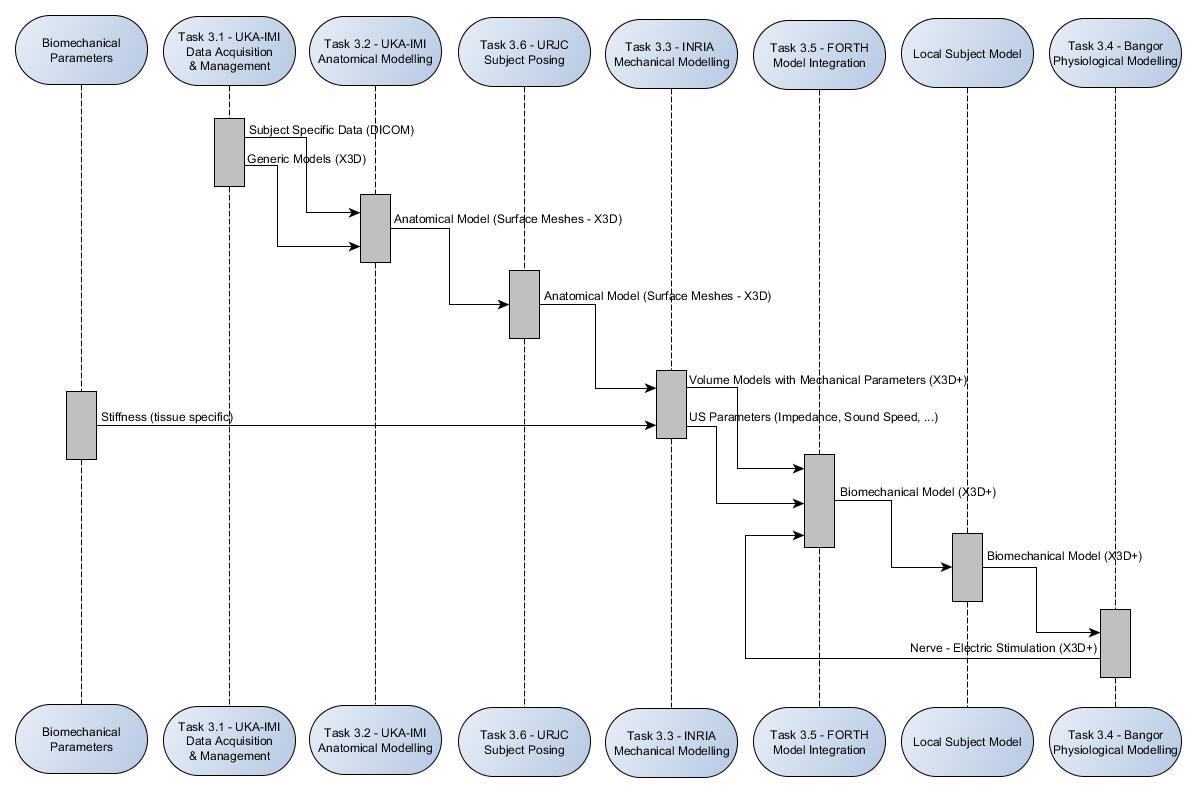
\includegraphics[width=0.5\textwidth]{IMG/RASimAs_D3.png}
%     \caption{ }
%   \label{fig:WP3}
% \end{figure}


% Por tanto, la tarea 3.6 necesita crear un método que sea capaz de modificar la posición de un paciente virtual a su posición final, de manera que pueda usar todos o varios resultados intermedios de las tareas anteriores a esta. Como parte de ese trabajo, esta tesis presenta una solución que se centra en resolver de manera innovadora los problemas encontrados.

% \todo{meter wp 5?}


%\todo{ En ese capitulo lo primero que tienes que contar es que este simulador da la opción de probar el posing. Permitiendo comprobar si los resultados son suficientemente buenos para ser usados para entrenamiento. Indicar que de cara a construir un simulador completo el proyecto se estructuro en paquetes de trabajos. Pon una sección donde expliques los paquetes de trabajo donde se desarrollaron los módulos relevantes del simulador y cual fue tu contribución a cada uno. En el resto del capitulo detalla esta contribución.}

El proyecto \ac{RASimAs} tiene como objetivo  facilitar el entrenamiento y la práctica de la \ac{RA} con la ayuda del simulador \ac{RASim} y el asistente \ac{RAAs}. El trabajo realizado en esta tesis ha estado centrado en el simulador.


Para fomentar su uso en el mayor número de sitios posibles (hospitales, universidades y colegios profesionales), se debe proporcionar una herramienta de entrenamiento que sea barata, fácil de usar, robusta y que necesite poco mantenimiento. Además, el simulador debe estar dirigido para diferentes perfiles de usuarios. Tanto estudiantes como profesionales que están empezando a realizar el procedimiento, el simulador les proporcionará un método de entrenamiento con el que mejorar sus habilidades cognitivas y propioceptivas. A su vez, este proyecto también está orientado para profesionales anestesistas que han estado alejados de la práctica del procedimiento y quieran retomar la actividad.


Se han definido unos objetivos principales del simulador \ac{RASim}:
\begin{enumerate}
    \item El estudiante puede adquirir y desarrollar las habilidades cognitivas y no cognitivas que le permitan ejecutar un bloque de nervio guiado por \ac{US} empezando por el bloqueo del nervio femoral y siguiendo con las siguientes localizaciones.
    \item Permitir a un anestesista retomar y practicar las habilidades necesarias para realizar el procedimiento de forma segura y satisfactoria.
    \item Recuperar y medir métricas de rendimiento al realizar el procedimiento en el simulador. 
    \item Permitir a un supervisor revisar las métricas registradas por los usuarios del simulador a través del tiempo.
\end{enumerate}



Como se introdujo en la sección \ref{intro:rasimas}, el proyecto \ac{RASimAs} se dividió en \acl{WP} (ver figura \ref{fig:wp_rasimas}) donde los \ac{WP} 3, 4 y 5 es donde se centraba el desarrollo de los prototipos \ac{RASim} y \ac{RAAs}. 
A continuación, se van a introducir brevemente las tareas de estos \acl{WP} y nombrar aquellos en los que ha contribuido de manera activa la \ac{URJC}, donde se encuadra la mayor parte de la investigación realizada en esta tesis. 

%\todo{vuelvo a poner la imagen?}

\begin{itemize}
%\todo{Frase mal redactada.  No has hablado de la importancia de crear una base de datos de pacientes. Recuerda resaltar que no se buscan pacientes reales sino pacientes promedio con distinta variabilidad.}
    \item 
El \ac{WP} 3 del proyecto \ac{RASimAs} tiene como objetivo crear la \emph{suite} \ac{ITGVPH}. Se integrará un conjunto de aplicaciones que servirán para generar una base de datos de \ac{VPH}, con el objetivo de conseguir un entrenamiento con una gran variabilidad anatómica. Además, se permite que el paciente virtual pueda ser adaptado a la postura que se requiera según el procedimiento que se esté realizando. Este paquete se ha dividido en las siguientes tareas:%Este paquete se divide en seis tareas lideradas por \ac{UKA-IMI}. }
\begin{enumerate}
    \item \textbf{Adquisición de datos:} análisis y recopilación de imágenes médicas que serán utilizadas para la creación de los \ac{VPH}.
    \item \textbf{Modelado anatómico:} se realiza un registro entre las imágenes médicas y modelos anatómicos comerciales con el objetivo de generar nuevos modelos anatómicos.
    Tanto la tarea anterior como esta fueron asignadas a \ac{UKA-IMI}.
    \item \textbf{Modelado mecánico:} se generan los modelos mecánicos que se utilizarán en la simulación física del simulador. Este módulo ha sido asignado al \ac{INRIA}.
    \item \textbf{Modelado fisiológico :} en esta tarea se modelará el comportamiento físico de los tejidos cuando los nervios son electroestimulados.
    Tarea asignada a \ac{Bangor}.
    \item \textbf{Herramienta de posicionamiento de pacientes:} este módulo permite adaptar la postura de los modelos anatómicos con todos sus tejidos asociados a la pose requerida por el simulador. Tarea desarrollada en \ac{URJC}, siendo la principal línea de investigación de la presente tesis. En esta tarea, se ha diseñado la aplicación \ac{TPTVPH} que será integrada dentro de la herramienta \ac{ITGVPH}.
    \item {\textbf{Integración:}
    esta tarea asignada a \ac{FORTH}, es la encargada de hacer la integración de todos los módulos anteriores en una única herramienta, ocultando los detalles técnicos a los futuros usuarios.}
\end{enumerate}
{Además de haber participado en las tareas asignadas a la \ac{URJC}, se ha participado activamente en la tarea 3.6, que se encarga de la comunicación de todas las tareas.}

% \begin{figure}[h]
%   \centering
%     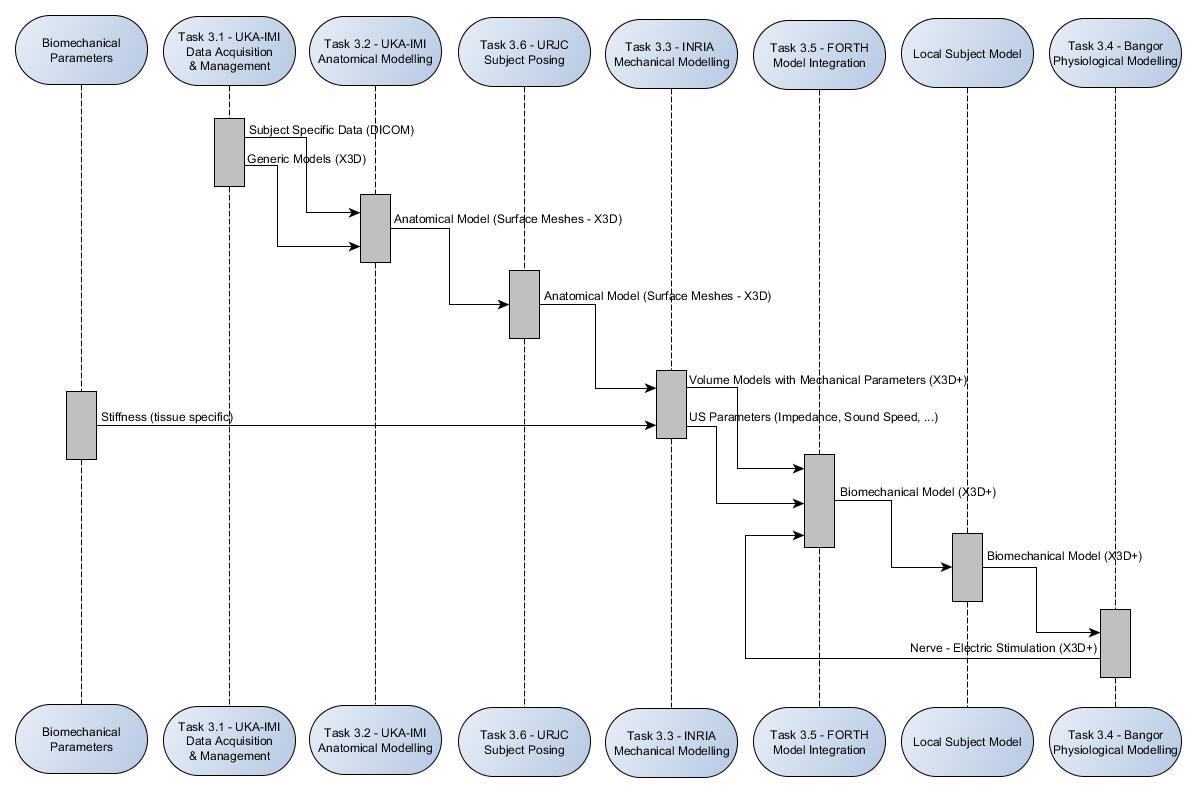
\includegraphics[width=0.9\textwidth]{IMG/RASimAs_D3.png}
%     \caption{ Diagramade secuencia que muestra la organización del \ac{WP} 3 }
%   \label{fig:WP3}
% \end{figure}
%Uno de los módulos clave es un posicionador \todo{no inventes palabras } de pacientes que sea capaz de deformar\todo{adaptar} modelos anatómicos que contengan todo tipo de tejidos \del{externos o internos} para adecuarlos a la posición requerida por el simulador.\todo{indicar cual es la pose de partida. No has dicho en ningún momento que se usan imagenes medicas en poses determinadas. No hables de pacientes reales, habla de imagenes medicas de pacientes reales}
 %\todo{indica el numero de la tarea y di que la lideró la URJC}
\item
El \ac{WP} 4 define las tareas para el desarrollo de los componentes que formarán parte de los prototipos de \ac{RASimAs}. Por una parte, los componentes pertenecientes a \ac{RASim} se definen en las tareas de la 1 a la 4. Por otra parte, la definición de los componentes del asistente \ac{RAAs} se realiza en las tareas 5 y 6. Estas tareas son las siguientes:

\begin{enumerate}
    \item \textbf{Retroalimentación háptica:}
    desarrollo del algoritmo que permite devolver una respuesta háptica al dispositivo que simula la aguja. Esta tarea fue asignada a \ac{INRIA}.
    \item \textbf{Simulación física:}
    este módulo desarrollado por \ac{INRIA} simula las deformaciones en los tejidos producidas por los instrumentos quirúrgicos.
    \item \textbf{Simulación de \ac{US}:}
    la \ac{RWTH} era la encargada de desarrollar el módulo que simulaba la generación de la imagen de \ac{US}.
    \item \textbf{Plataforma de entrenamiento:}
    esta aplicación se comunicaba con todos los módulos anteriores con el objetivo de proporcionar una aplicación de entrenamiento y autoevaluación. Esta tarea fue asignada a la \ac{URJC}. Esta tarea es una de las contribuciones de esta tesis.
    \item \textbf{Modelado en tiempo real:} esta tarea, perteneciente a \ac{RAAs}, se basa en reconstruir un modelo virtual a partir de las imágenes de \ac{US}. El asistente \ac{RAAs} mostrará estos modelos como ayuda adicional en el procedimiento.
    \item \textbf{Guiado en el procedimiento:}
    el asistente proporcionará ayuda al anestesista durante la intervención, ya que el sistema muestra información sobre la imagen de \ac{US}.
    Tanto la tarea anterior como esta fueron asignadas a \ac{SINTEF}.
\end{enumerate}

Debido a la importancia del \ac{Courseware}, el autor de esta tesis ha participado en las tareas 1, 2, y 3. Este módulo se comunica y gestiona con todos los módulos del simulador.%La importancia de la plataforma de entrenamiento ha dado lugar a participar en las tareas 1, 2 y 3 debido a que el \ac{Courseware} se comunica y gestiona todos los módulos de \ac{RASim}.

%\todo{Indica las tareas y en cuales has estado involucrado. Indicar cuales se han liderado.}

\item
El \ac{WP} 5 se centra en la integración y desarrollo los prototipos del simulador \ac{RASim} y el asistente \ac{RAAs}. %En el \ac{WP} 6 El objetivo es crear los prototipos con intención de comprobar su validez en evaluaciones clínicas (\ac{WP} 6) con vistas a su posterior comercialización.
\begin{itemize}
    \item {\textbf{Tareas 1 y 2: } integración y construcción del prototipo \ac{RASim} a cargo de \ac{SG}. 
    }
     \item {\textbf{Tareas 3 y 4: } integración y construcción del prototipo del asistente \ac{RAAs} a cargo de \ac{SINTEF}.
    }
\end{itemize}

{Al igual que el \ac{WP} anterior, la importancia del \ac{Courseware} en el prototipo \ac{RASim} hace que se haya trabajado conjuntamente con \ac{SG} para el desarrollo e integración de todos los módulos del simulador. También se contribuyó al proponer una solución con \acs{tracker}s magnéticos ante los problemas encontrados con los dispositivos hápticos.}



\end{itemize}
